\documentclass[12pt,a4paper,twoside]{article}
\usepackage{amsmath,amsfonts,amssymb}
\usepackage{graphicx}
\usepackage{url}
\usepackage[left=2.00cm,right=2.00cm,top=2.00cm,bottom=2.00cm]{geometry}

\begin{document}

	\begin{center}
		\begin{large}
			\textbf{BUILD AN EXERCISE SUPPORTER APP WITH OPENCV AND CONVOLUTIONAL NEURON NETWORKS}\\
		\end{large}
	\end{center}

	\begin{flushleft}	
		\textbf{I. INTRODUCTION}
			\begin{flushleft}
		Social distancing and working from home help prevent transmission of the coronavirus (COVID-19) but can be conducive to unhealthy behavior such as bingeing on either fast food or soft drink, and spending more time on a couch staring at a screen, being a couch potato. Overally moving about less during the day. Scientists believe the reduction in physical activity experienced during the first few months of the pandemic could lead to an annual increase of more than 11.1 million in new cases of type 2 diabetes and result in more than 1.7 million deaths.\\
		\medskip
		Vietnam generally is known as a country with below average health status. Due to the widespread of the disease, people need to start woking out in order to improve their health against this pandemic. One of the most effective work out excercise to improve your strength that you can do at home so far is push up. However, it doesn't seem like we all know how to do it in the proper way, which is the main reason for us to develop this project.
			\end{flushleft}
	\end{flushleft}

	\begin{flushleft}
		\textbf{II. RELATED WORK}
			\begin{flushleft}
		Formerly, there was a push-up project, but it main task is to count how many times a person push up but doesn't recognise whether the person is doing push up in the correct or incorrect form.\\
		Link: \url{https://aicurious.io/posts/2021-02-15-build-a-pushup-counter/}
			\end{flushleft}
	\end{flushleft}

	\begin{flushleft}
		\textbf{III. DATA PREPARATION}
			\begin{flushleft}
		Because this project is contemporary, there is a limitation in data, so we have to collect more by using our own data, and then label them alternately.\\
		\smallskip
		Data is classified into 2 categories:\\
		+ Up: Taken while the person is pushing up on the highest, both arms are straight and perpendicular to the ground.\\
		+ Down: The opposite of up, taken while the person is doing push up on the lowest, each arm make up a smallest acute angle.\\
		\smallskip
		For each categories, there are also 2 classes:\\
		+ Right: Person doing push up in the correct form.\\
		+ Wrong: Person doing push up in the incorrect form.\\
		\smallskip
		Total: 3300 images\\
		+ Collect from the Internet: 20\% (images, or crop frames from multiple videos)\\
		+ Self made: 80\% (5 different person)\\
		\begin{center}
			\begin{tabular}{ |c|c|c|c|c| } 
 				\hline
 				Up & Right & 900 images & \includegraphics[width=0.3\textwidth, height=30mm]{images/img001.png} & 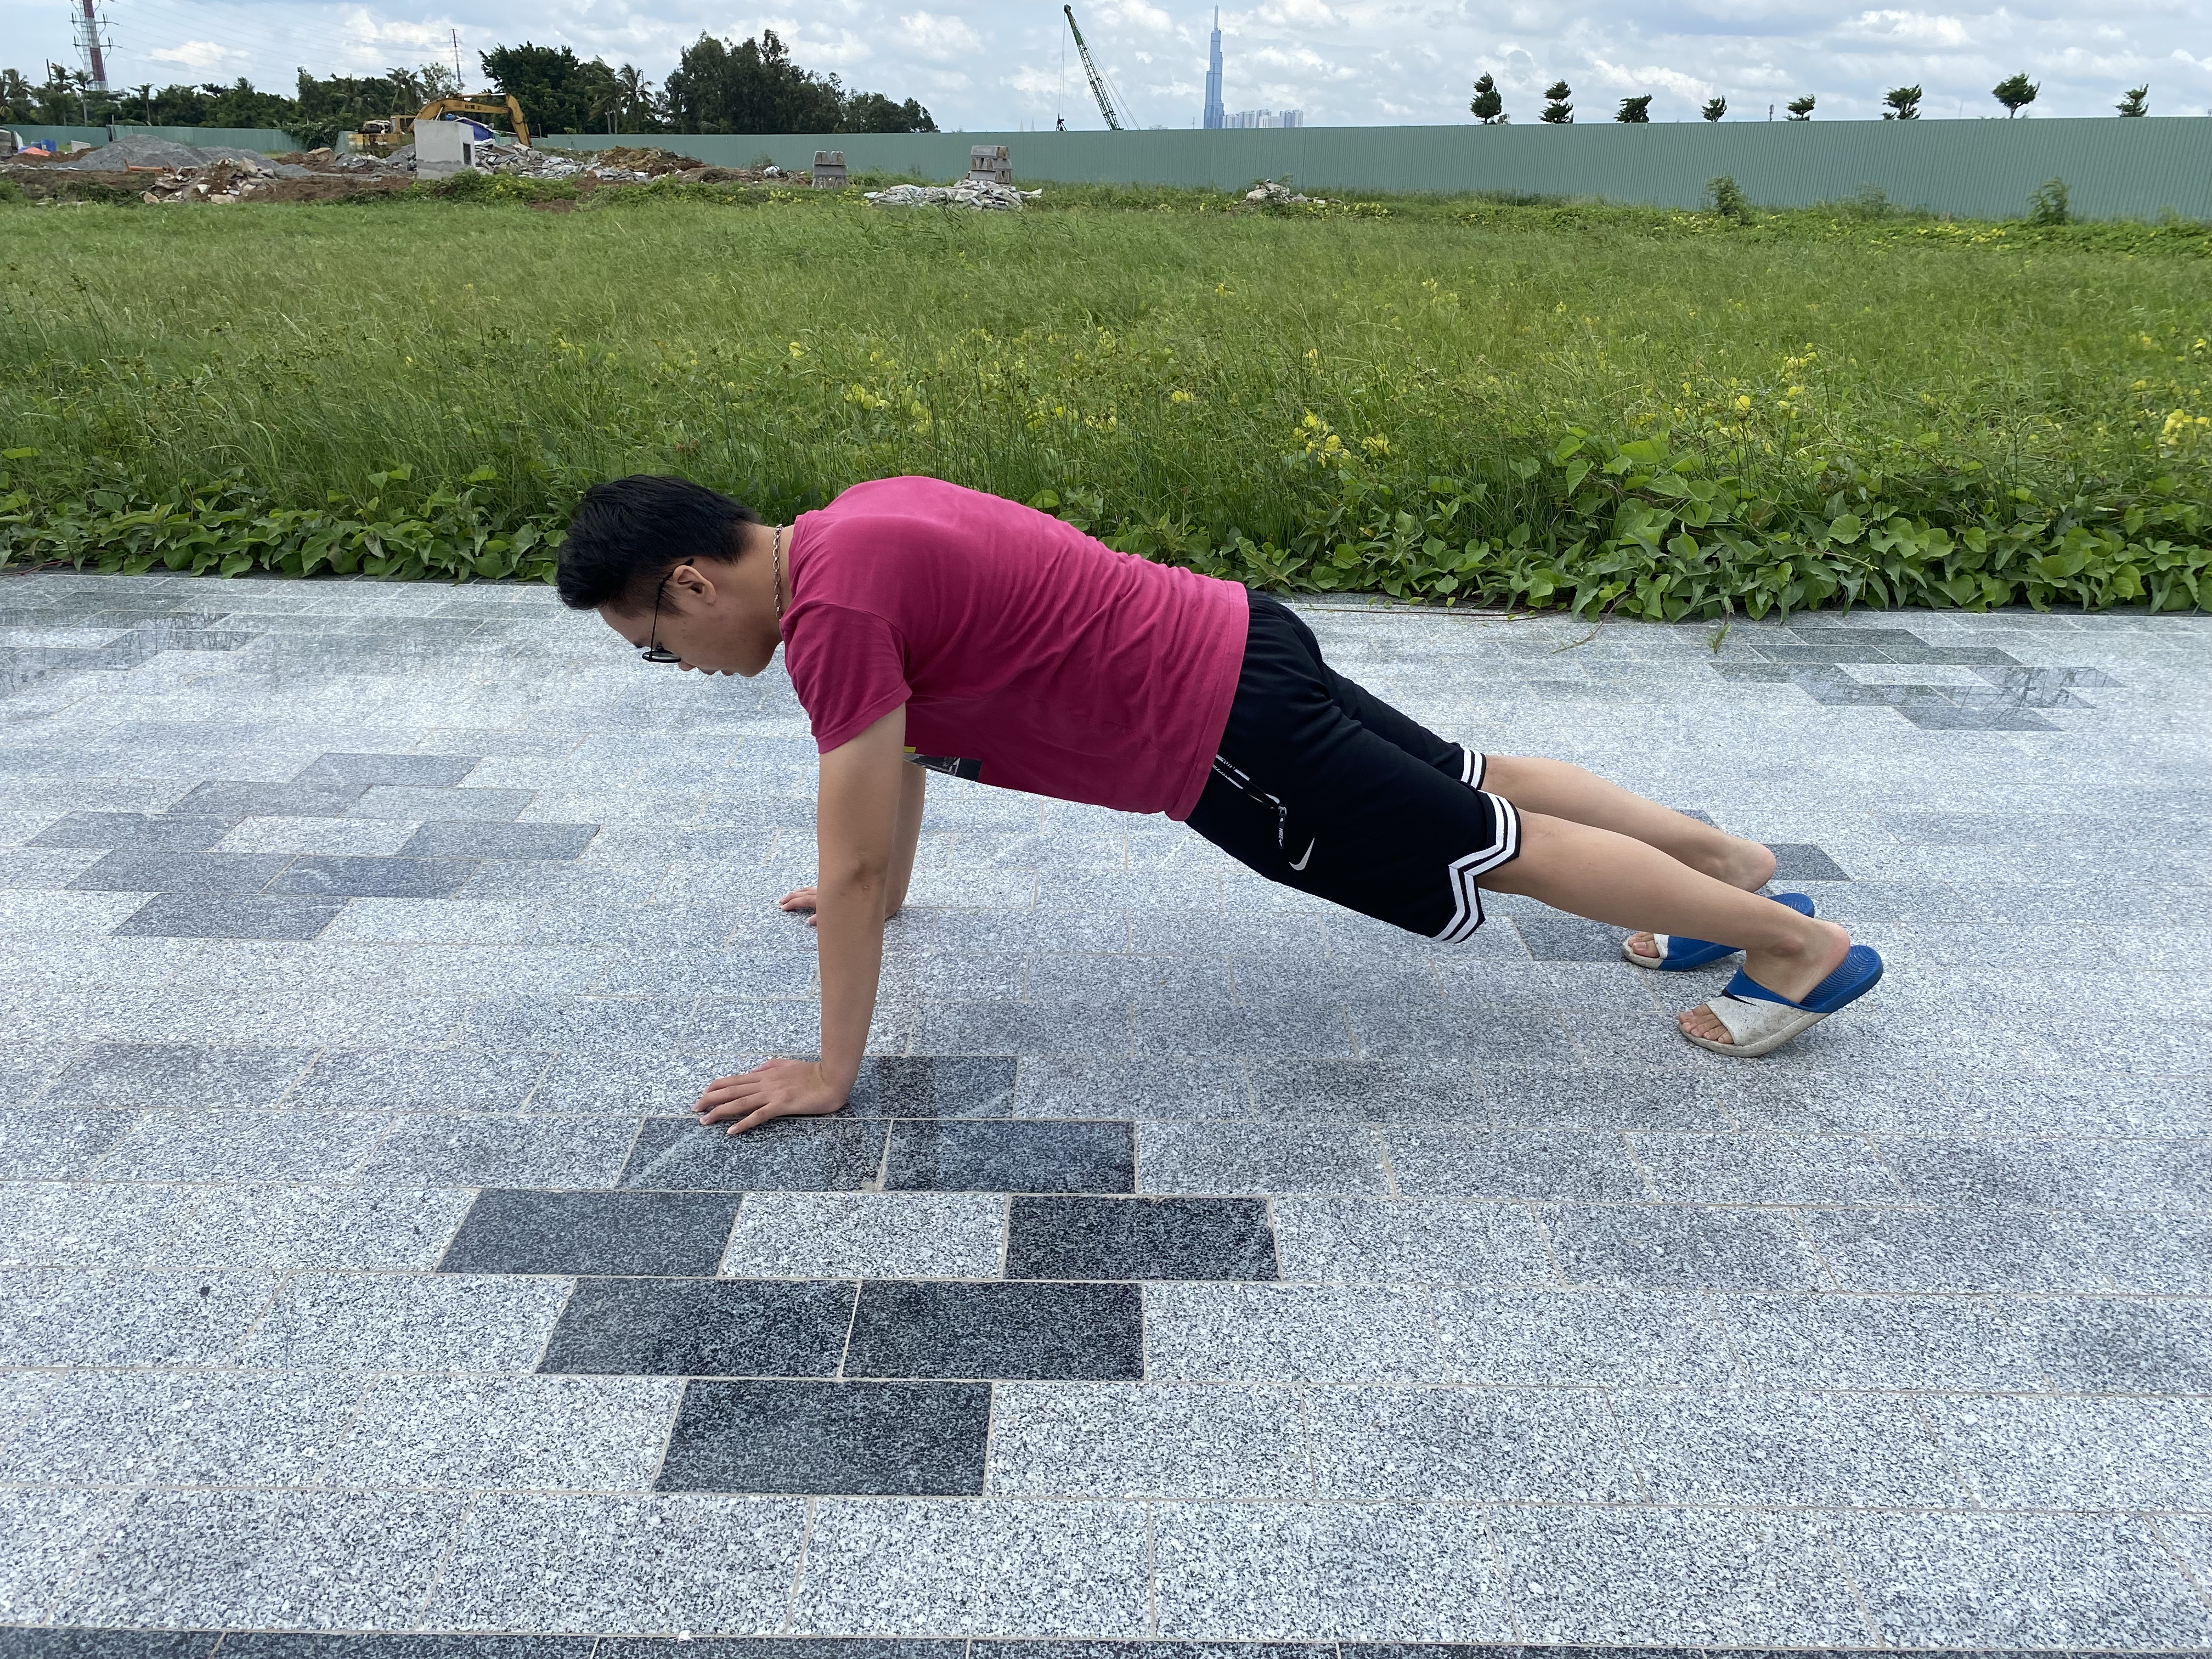
\includegraphics[width=0.3\textwidth, height=30mm]{images/img002.jpg}\\ 
 				& Wrong & 900 images & 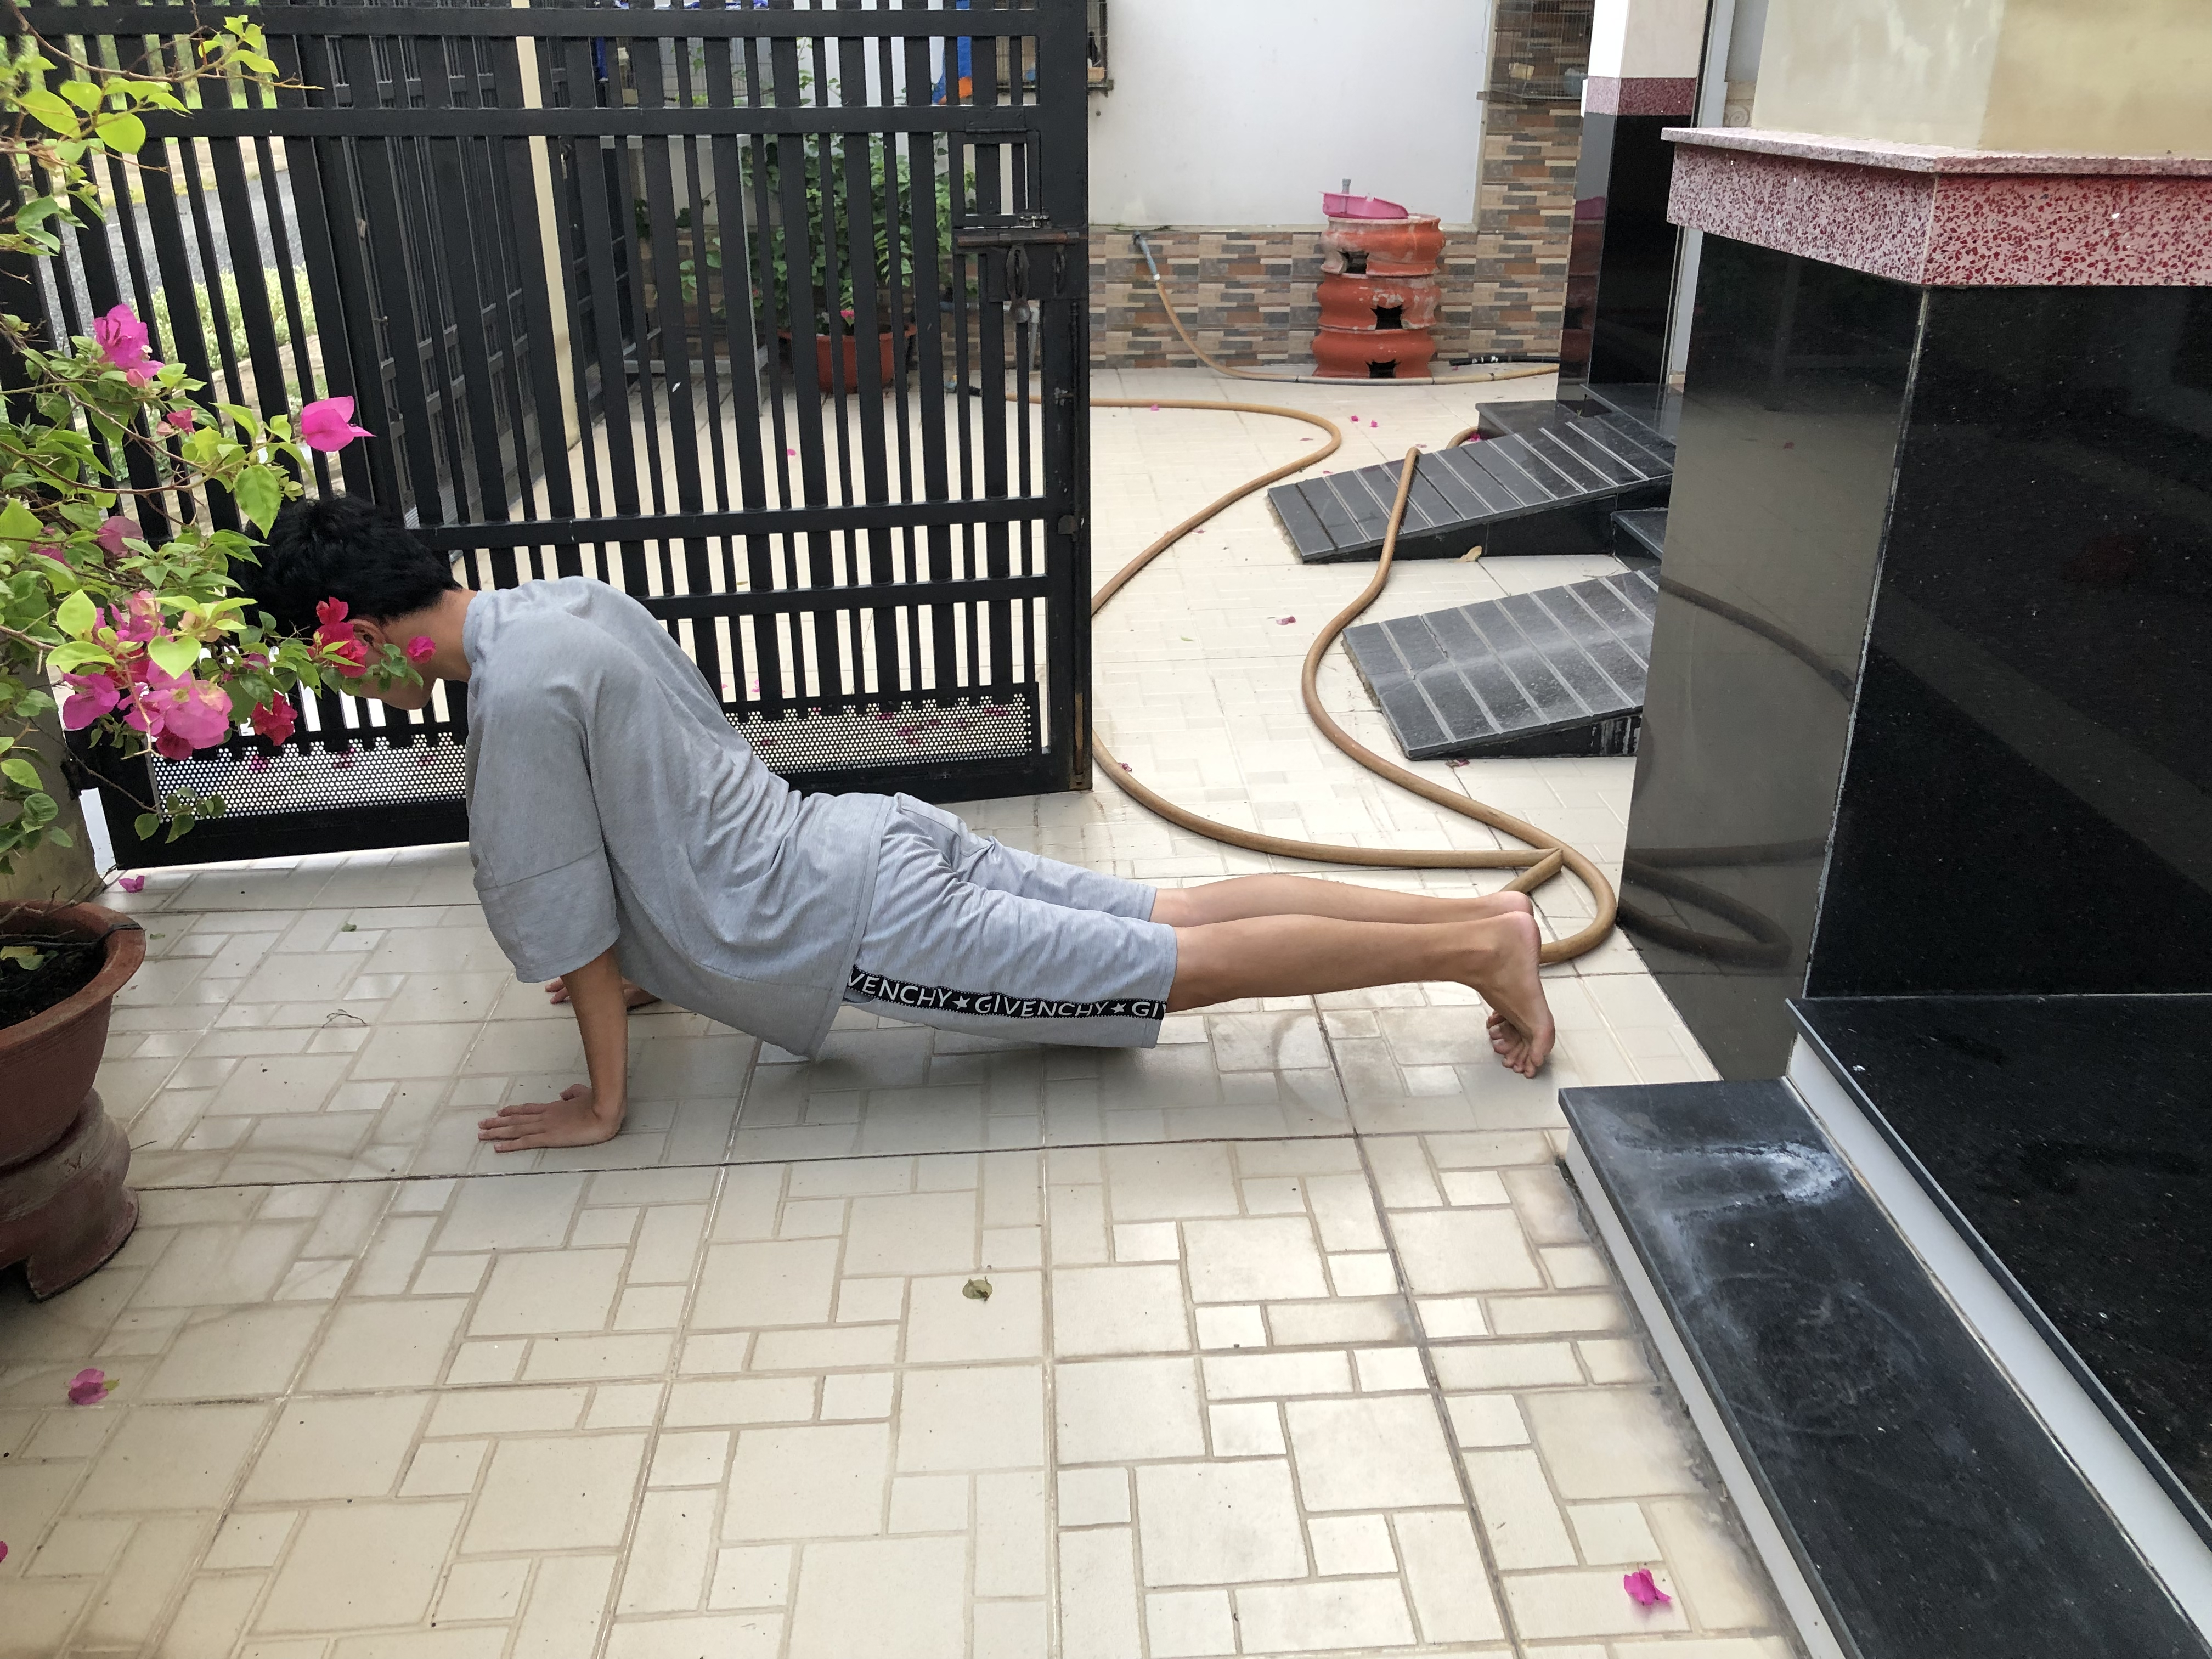
\includegraphics[width=0.3\textwidth, height=30mm]{images/img003.jpg} & \includegraphics[width=0.3\textwidth, height=30mm]{images/img004.png}\\ 
 				\hline
 				Down & Right & 750 images & \includegraphics[width=0.3\textwidth, height=30mm]{images/img005.png} & 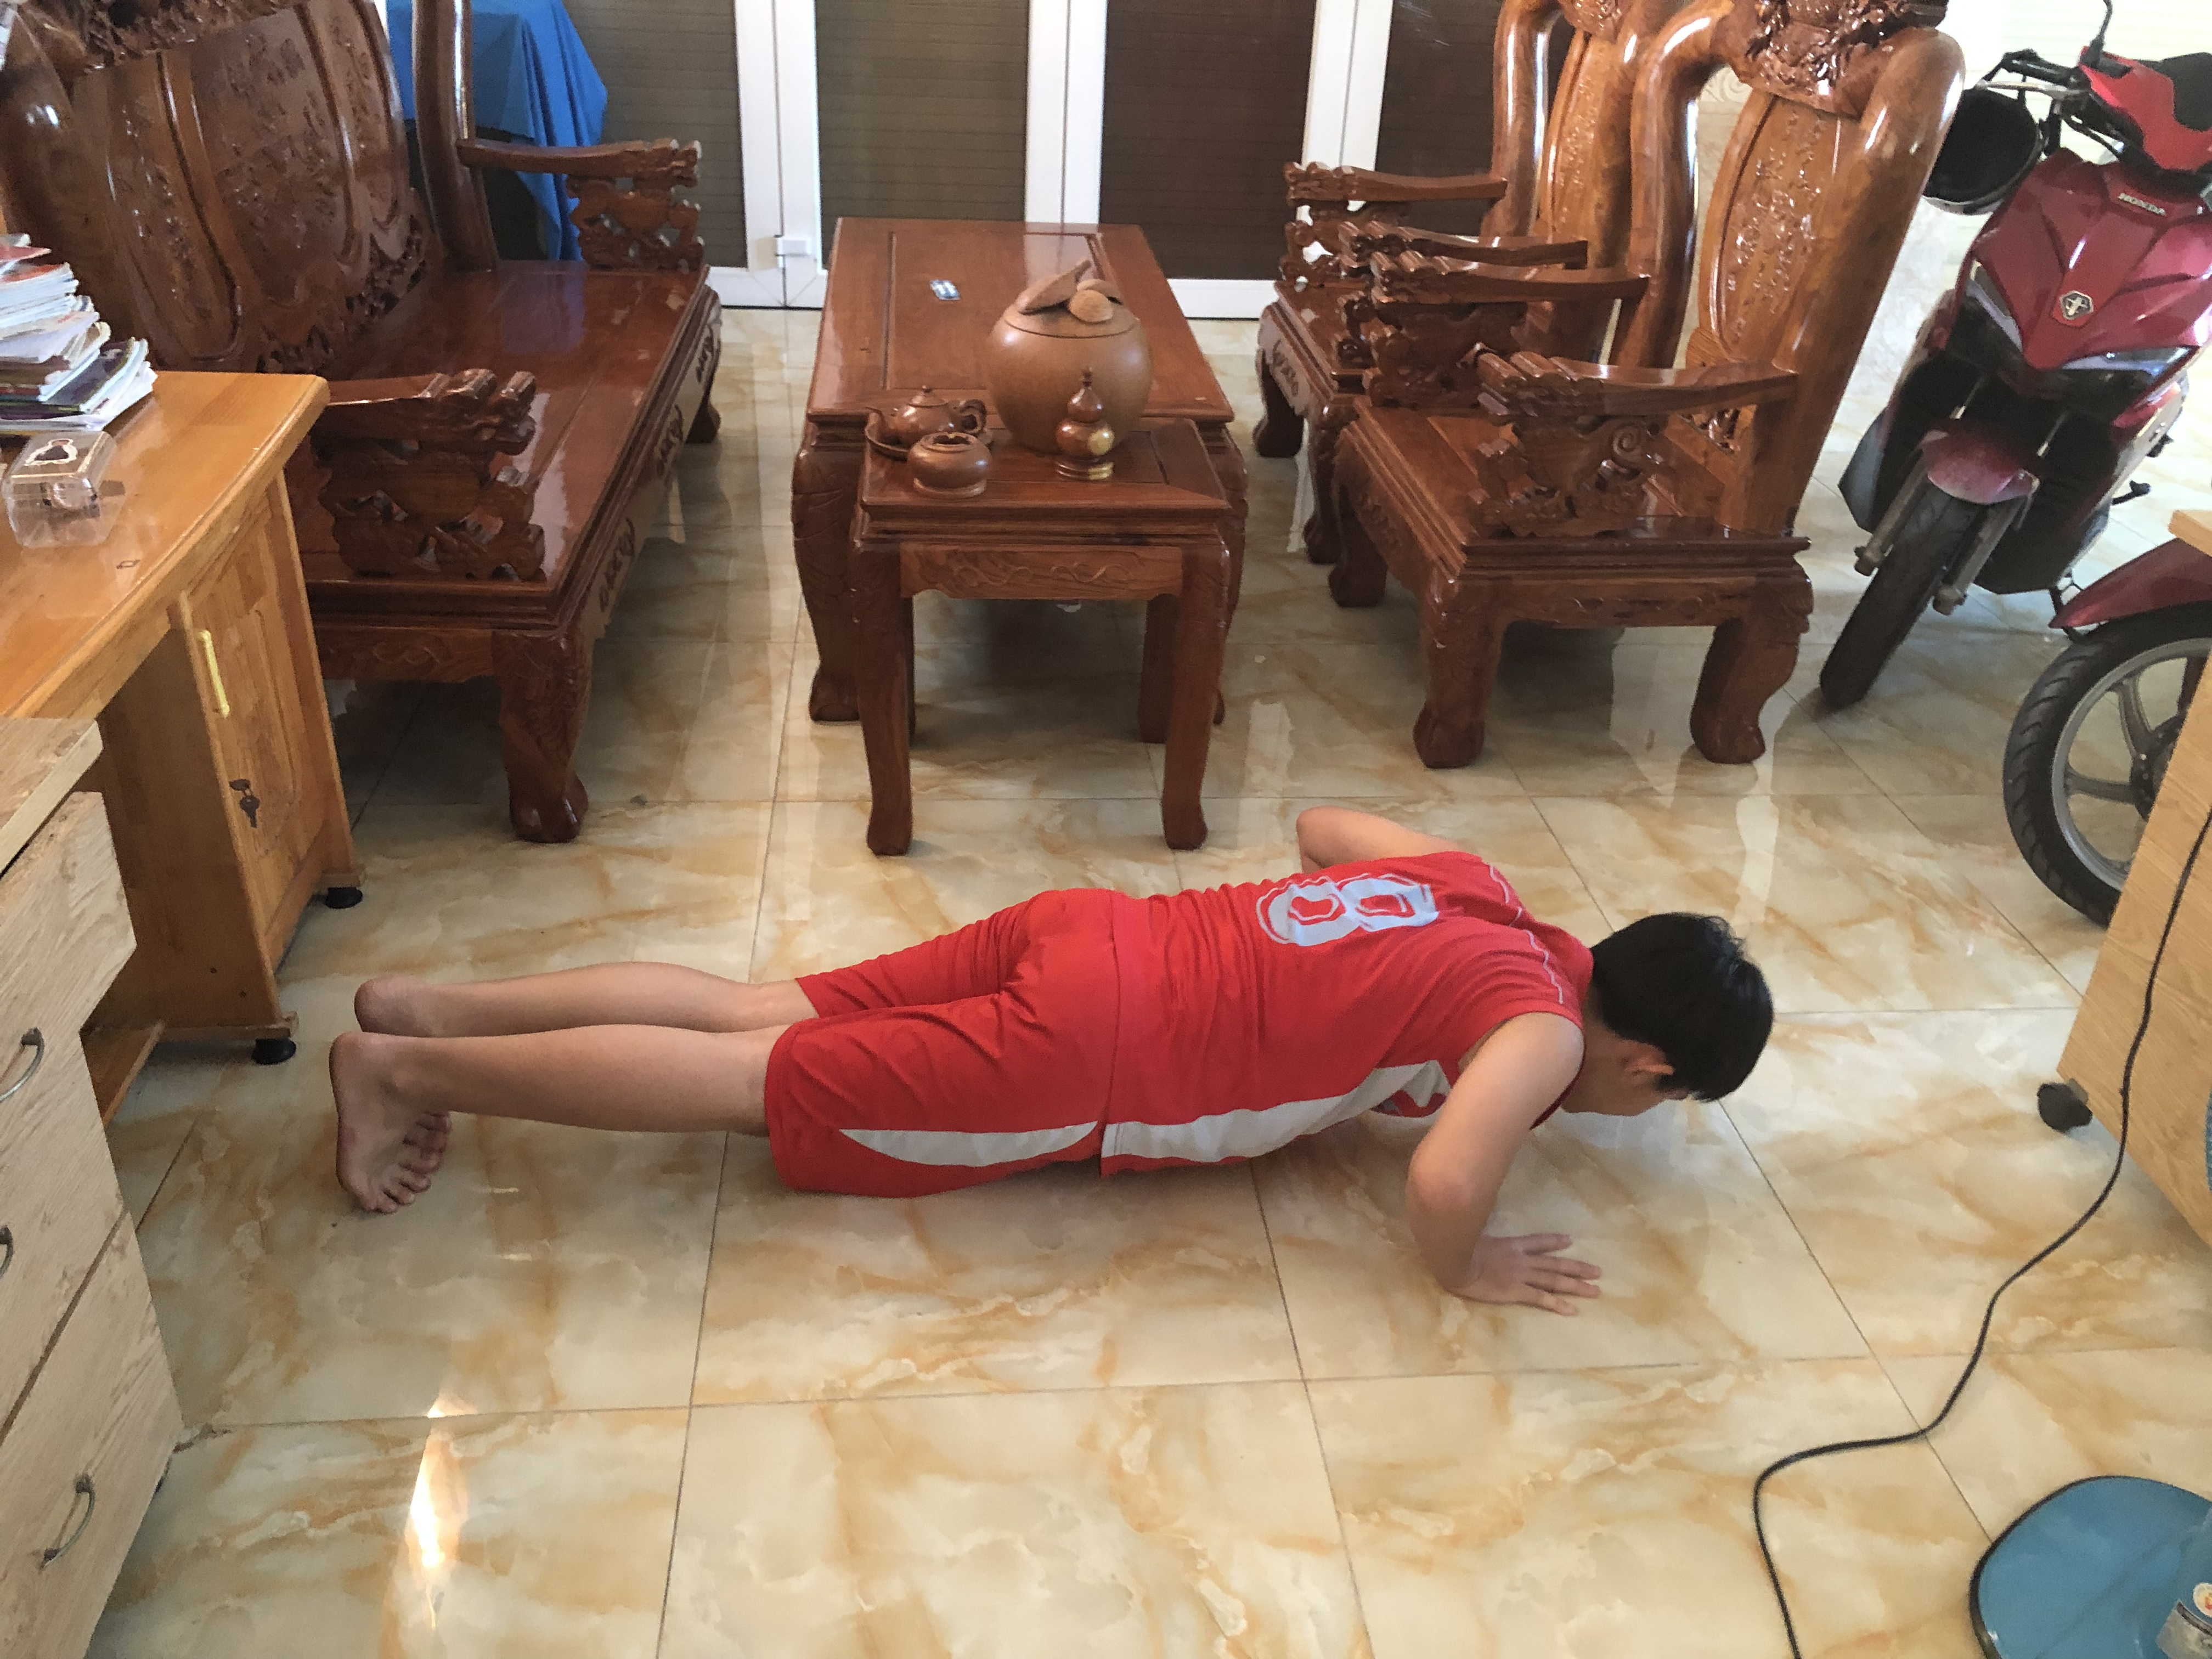
\includegraphics[width=0.3\textwidth, height=30mm]{images/img006.jpg}\\ 
 				& Wrong & 750 images & 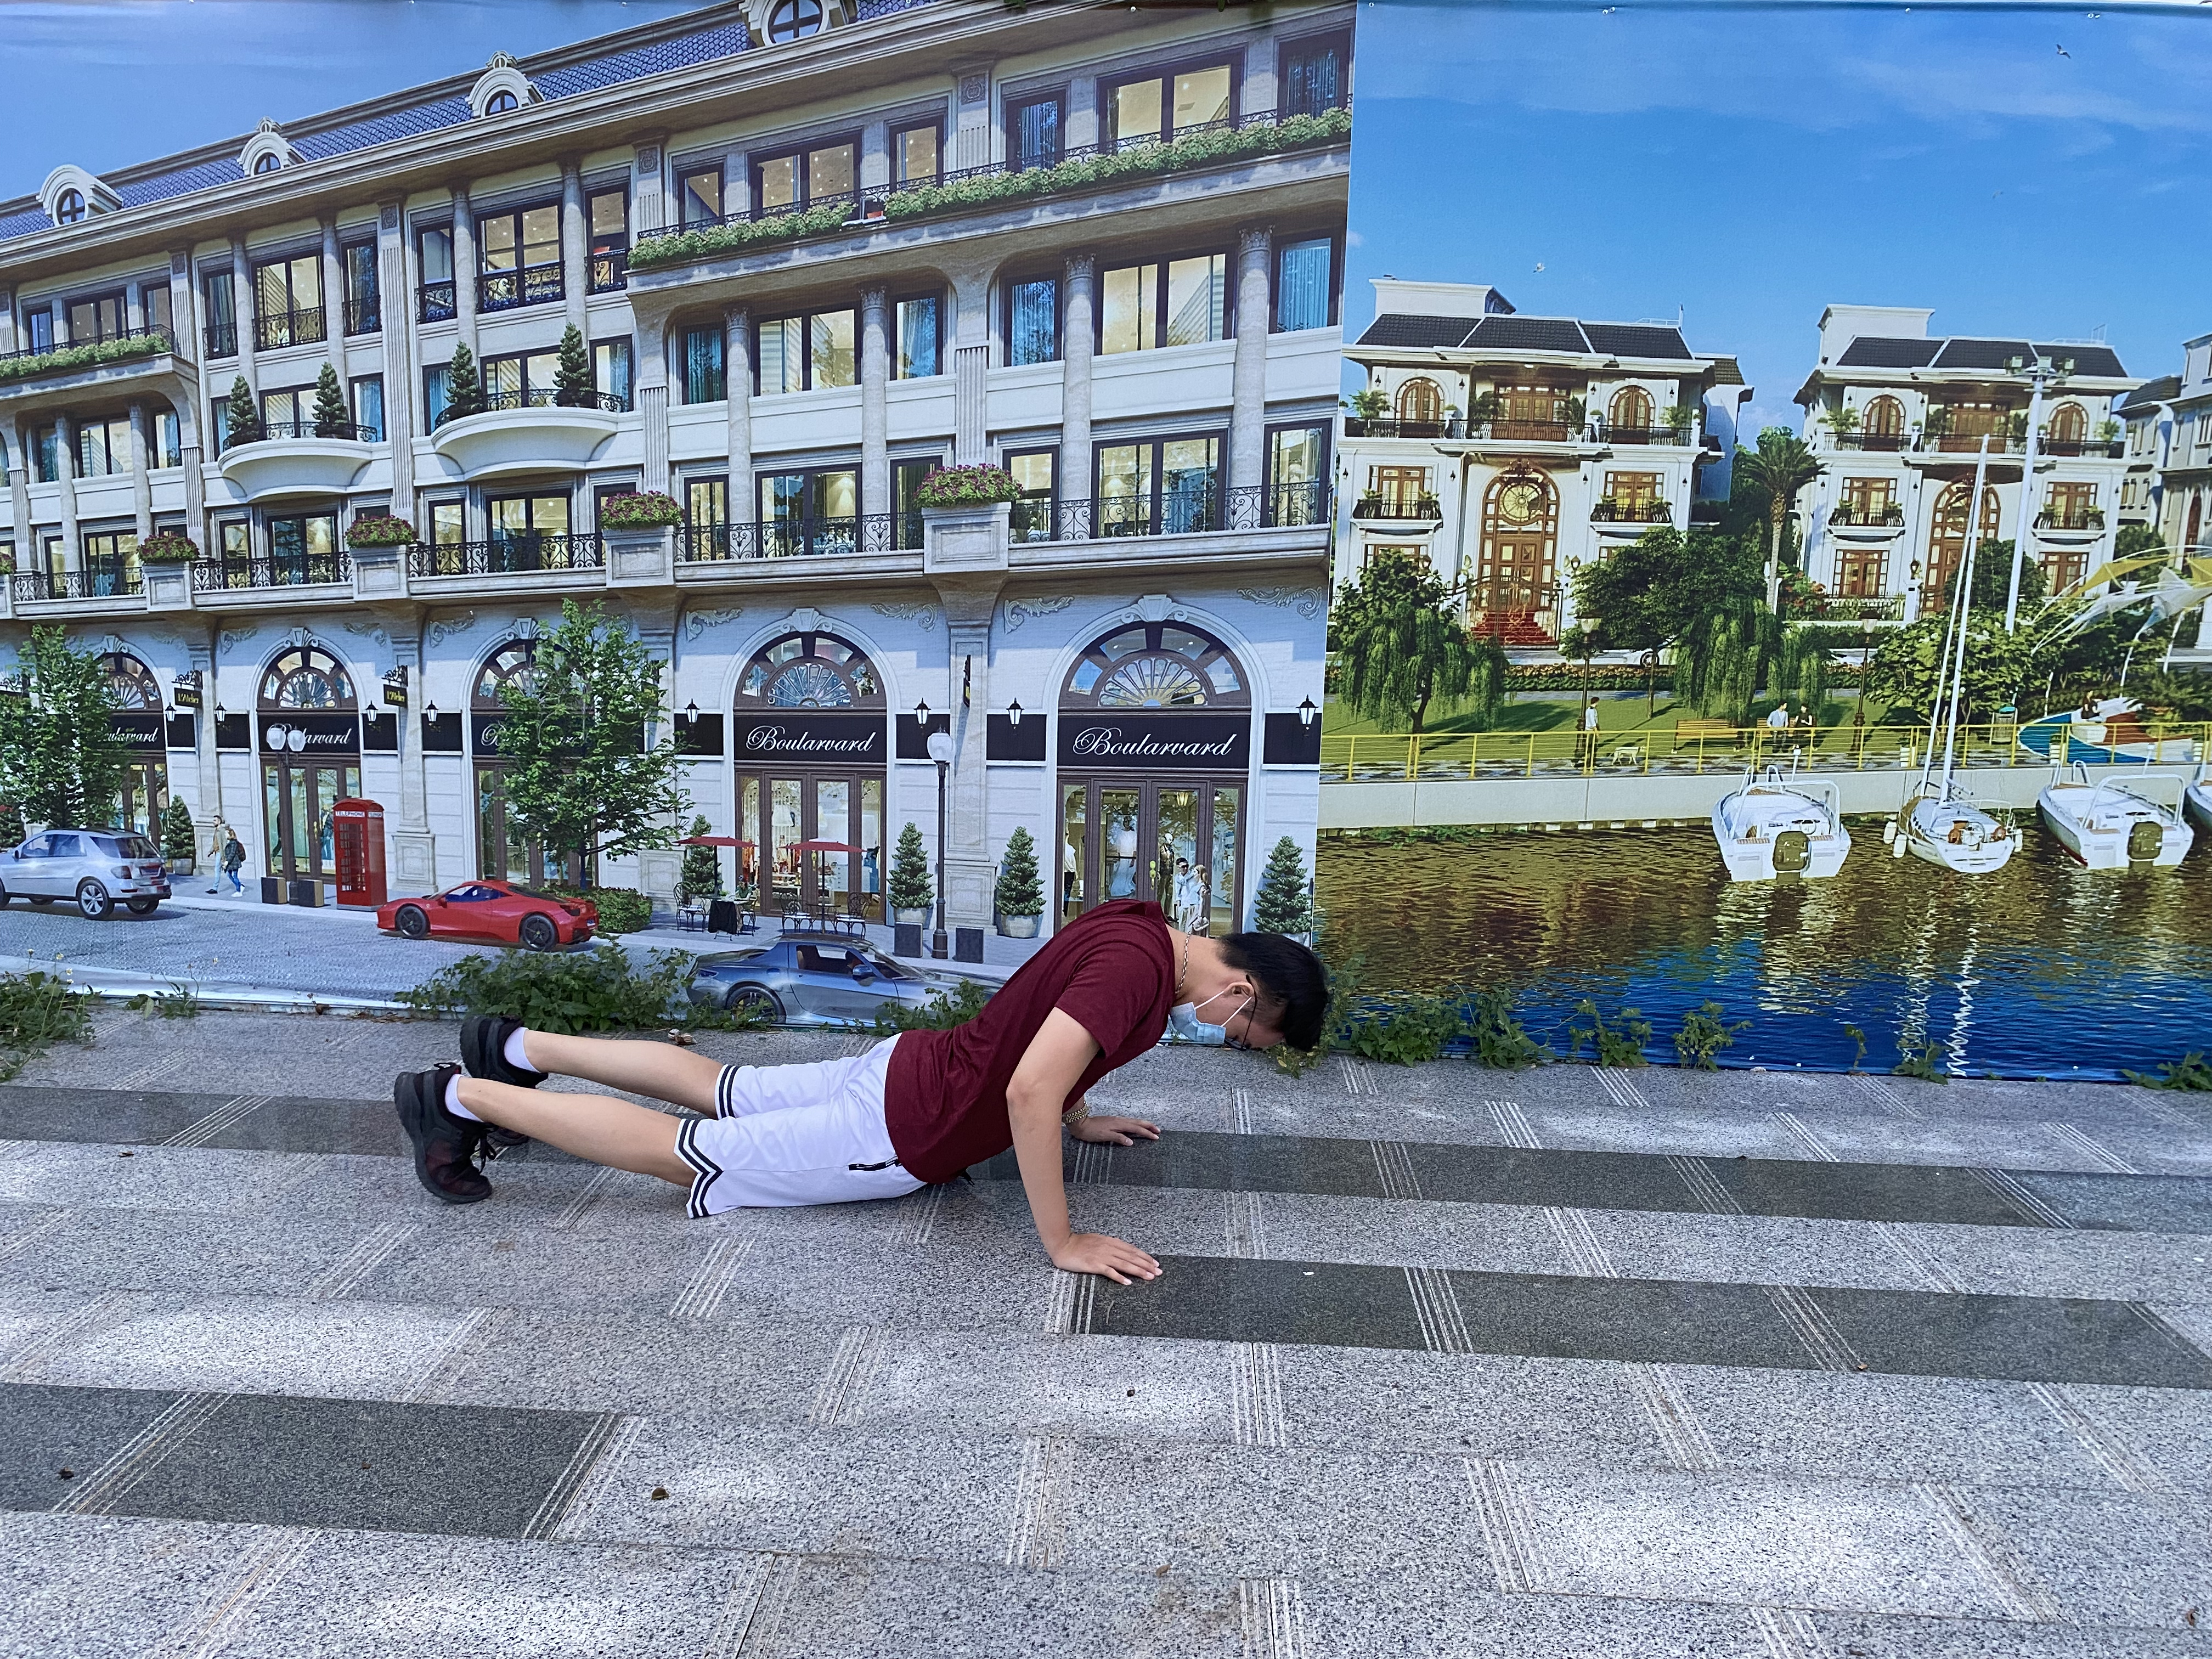
\includegraphics[width=0.3\textwidth, height=30mm]{images/img007.jpg} & \includegraphics[width=0.3\textwidth, height=30mm]{images/img008.png}\\
 				\hline
		\end{tabular}
\end{center}
			\end{flushleft}
	\end{flushleft}
	\bigskip
	\begin{flushleft}
		\textbf{IV. METHOD}
			\begin{flushleft}
			\medskip
			(insert image later)\\
			\medskip
		Steps:\\
		\smallskip
		1. Using Mediapipe to locate 3 bodyparts: shoulder, elbow and wrist.\\
		2. Calculate the angle formed by 2 sides: shoulder - elbow and elbow - wrist.\\
		3. Using signal processing (low-pass filter) to count push-ups detected in frame.\\
		4. In each push-up, extract 2 frames at the highest and lowest angle measurements, corresponding to ups and downs.\\
		5. Use 2 different models (Efficient Net and Transfer Learning with 4 Dense layers interleaved and Droupout) to evaluate whether the person's push up form in those 2 frames are correct or incorrect.\\
		6. A push-up is correct when both up and down are right, if one of the two is wrong, it is considered a wrong push-up.\\
			\end{flushleft}
	\end{flushleft}
	\bigskip
	\begin{flushleft}
		\textbf{V. METRICS: ACCURACY AND CONFUSION MATRIX }
		\begin{flushleft}
			\begin{flushleft}
			- Model up: Accuracy: 90\%
			\medskip
			\end{flushleft}
			\begin{tabular}{ |c|c|c| }
				\hline
 				& Possitive & Negative \\ 
 				\hline
 				True & X & X \\  
 				False & X & X \\ 
 				\hline  
			\end{tabular}
		\end{flushleft}
		\begin{flushleft}
			\begin{flushleft}
			- Model down: Accuracy: 85\%
			\medskip
			\end{flushleft}
			\begin{tabular}{ |c|c|c| }
				\hline
 				& Possitive & Negative \\ 
 				\hline
 				True & X & X \\  
 				False & X & X \\ 
 				\hline  
			\end{tabular}
		\end{flushleft}
		\begin{flushleft}
			\begin{flushleft}
			- Combined two models: Accuracy: \%
			\medskip
			\end{flushleft}
			\begin{tabular}{ |c|c|c| }
				\hline
 				& Possitive & Negative \\ 
 				\hline
 				True & X & X \\  
 				False & X & X \\ 
 				\hline  
			\end{tabular}
		\end{flushleft}
	\end{flushleft}
	\bigskip
	\begin{flushleft}
		\textbf{VI. SUMMARY AND FUTURE PLANS}
		\begin{flushleft}
		Pros:\\
		+\\
		Cons:\\
		+ Unable to perform detection if the person's head is facing the camera directly.\\
		+ 95\% of the data used for training is male.\\
		+ Self-made dataset despite having a variety of costumes and backgrounds, but only created from 5 different people. Althrough the pretrained model (Efficient Net) has peak performance in extracting information on a person's body, but it will still be less effective in extracting information of other different people.\\
		+ Partially dependent on Mediapipe, it will not be able to recognize and evaluate if Mediapipe does not recognize the person's poses.\\
		+ Only inform people whether their form is currently correct or incorrect but not giving out the reason why.\\
		\bigskip
		Future works to improve results:\\
		+ Collect more variety data to avoid gender bias, race bias.\\
		+ Expand 'Wrong' class of each model, 'Wrong', 'Wrong Reason1' , 'Wrong Reason2', 'Wrong Reason3', etc. Moreover, specify problem 'Why the pushup is wrong?'.\\
		\end{flushleft}
	\end{flushleft}
	\bigskip
	\begin{flushleft}
		\textbf{VII. REFERENCES}\\
		\medskip
		- Build a Pushup counter app with OpenCV and DeepLearning
		\url{https://aicurious.io/posts/2021-02-15-build-a-pushup-counter/}\\
		\medskip
		- Deep Learning Exercise repeatitions Counter
		\url{https://github.com/NetoPedro/Deep-Learning-Push-Up-Counter}\\
		\medskip
		- Mediapipe Pose
		\url{https://google.github.io/mediapipe/solutions/pose}\\
		\medskip
		- Low pass filter algorithm, Wikipedia
		\url{https://en.wikipedia.org/wiki/Low-pass_filter}\\
		\medskip
		- Efficient Net, Rethinking Model Scaling for Convolutional Neuron Networks
		\url{https://arxiv.org/pdf/1905.11946.pdf}
	\end{flushleft}
	\bigskip
	\begin{flushleft}
		\textbf{VII. APPENDIX}
	\end{flushleft}

\end{document}